\documentclass{beamer}
\usetheme{Warsaw}
\usecolortheme{beaver}
\usepackage{polski}

\usepackage{multimedia}
\usepackage{media9}

\title{Prezentacja do Projektu}
\subtitle{Eksploracja i wizualizacja danych}
\author{Michał Brodacki, s32038}
\institute{Polsko--Japońska Akademia Technik Komputerowych}
\date{16 Grudnia 2023}

\usepackage{geometry}
\usepackage{graphicx}
\usepackage{subcaption}
\begin{document}
	\begin{frame}
		\titlepage
	\end{frame}
	\begin{frame}{Spis Treści}
		\tableofcontents % Slajd ze spisem treści
	\end{frame}
	
	\section{Cel i Dane}
	\subsection{Cel}
	\begin{frame}
		\begin{block}{Cel Projektu}
		Celem projektu jest rozpoznanie na podstawie danych pozycyjnych koszykarza oddającego rzut, czy będzie on liczony jako $3$--punktowy, czy jako $2$--punktowy.
		\end{block}

	\end{frame}
	\subsection{Dane}
\begin{frame}
	\frametitle{Dane}
Do projektu wykorzystam dane NBA 2023 Player Shot Dataset dostępne pod linkiem: 
\textit{\url{https://www.kaggle.com/datasets/dhavalrupapara/nba-2023-player-shot-dataset/?select=2_james_harden_shot_chart_2023.csv}}. Zawierają one informacje na temat sytuacji rzutowych trzech koszykarzy występujących w \textbf{NBA}.
\end{frame}
\begin{frame}
	\begin{center}
		\includegraphics[width=11cm, height=4cm]{dane.png}
	\end{center}
\end{frame}
	\subsection{Wstępna ocena danych}

\begin{frame}
	\frametitle{Wstępna ocena danych}
		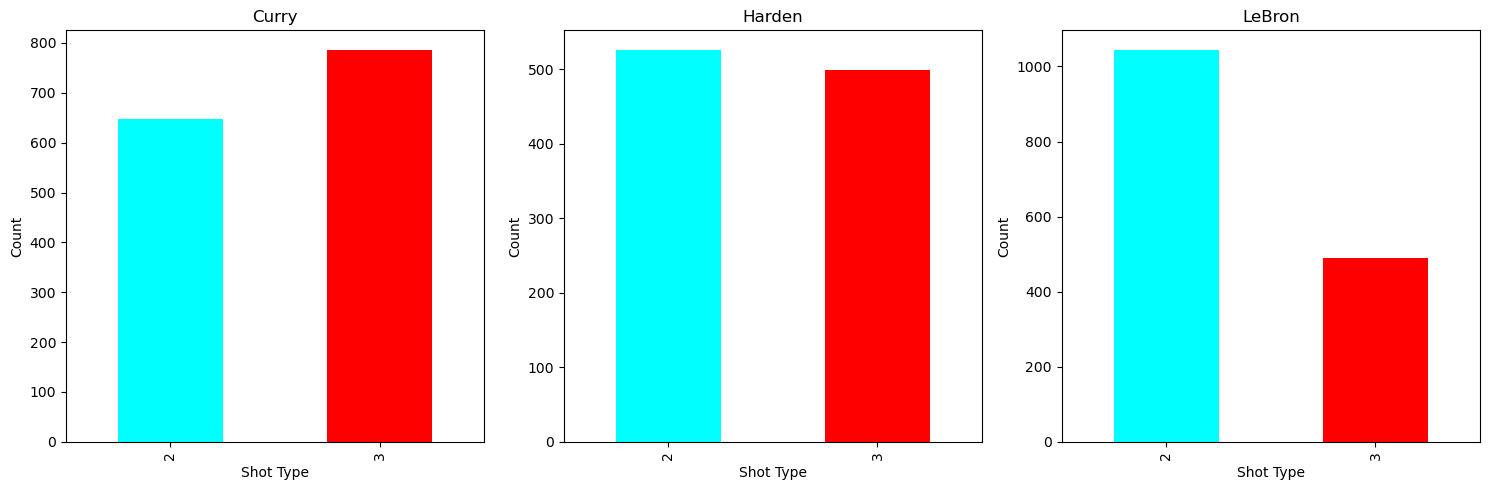
\includegraphics[width=\linewidth]{WstepnaOcena1.png}


		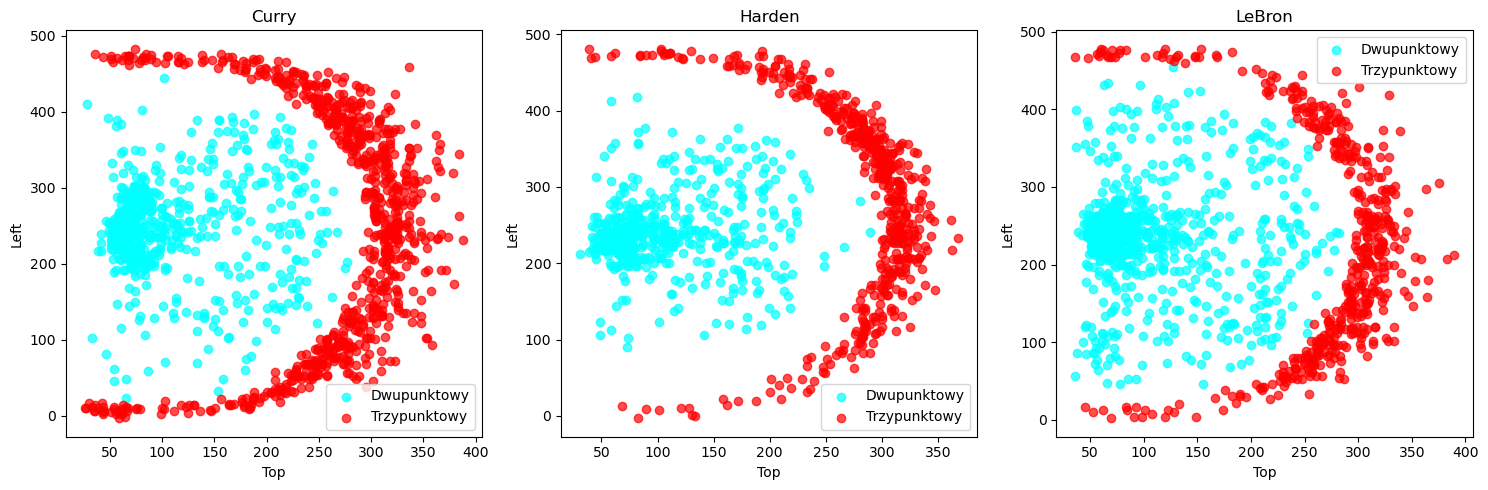
\includegraphics[width=\linewidth]{WstepnaOcena2.png}

\end{frame}
\subsection{Przygotowanie Danych}
	\begin{frame}
		\frametitle{Przygotowanie Danych}
		Na tym etapie wykonane zostały następujące czynności:
		\begin{itemize}
			\item Sprawdzono czy zbiór danych zawiera brakujące wartości \pauza nie zawiera
			\item Zbadano kodowanie zmiennej, która będzie później estymowana \textit{Curry["shot\_type"].dtype} i wyszło \textit{dtype('int64')}.
			\item Na potrzeby klasyfikacji stworzono nową zmiennę \textit{is\_three}
, którą zastąpiono zmienną \textit{shot\_type} (zmienna typu Bool).
\item Podzielono zbiór na częsci: treningową, walidacyjną i testową na dwa sposoby:
\begin{enumerate}
	\item W pierwszej wersji rzuty jednego zawodnika stanowiły zbiór treningowy, drugiego walidacyjny, a trzeciego testowy.
	\item W drugiej złączono wszystkie \textit{dataframe'y} i podzielono na trzy zbiory całość.
\end{enumerate}
		\end{itemize}
		
	\end{frame}
	\section{Model}
	\subsection{Modelowanie}
\begin{frame}
	\frametitle{Modelowanie}
	\begin{figure}
		\begin{subfigure}[b]{0.49\textwidth}
			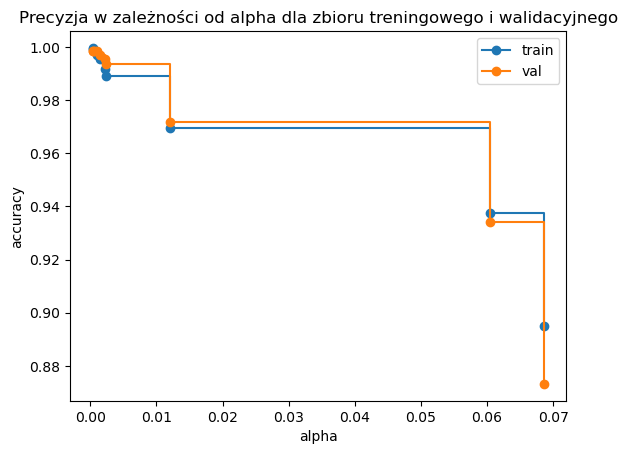
\includegraphics[width=\linewidth]{ModelowanieTree.png}
		\end{subfigure}
		\begin{subfigure}[b]{0.49\textwidth}
			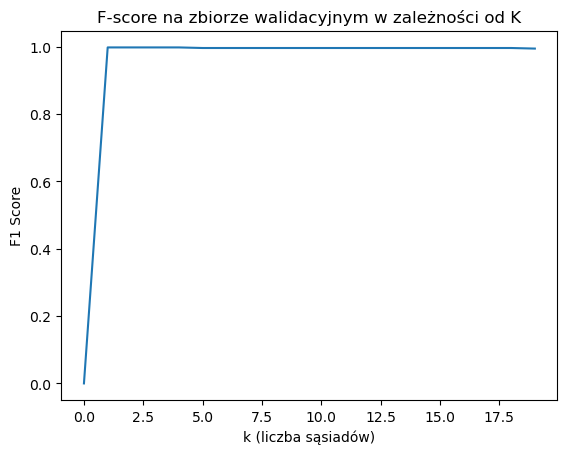
\includegraphics[width=\linewidth]{ModelowanieKNN.png}
		\end{subfigure}
	\end{figure}
\end{frame}
	\subsection{Ewaluacja}

\begin{frame}
	\frametitle{Regresja Logistyczna}
	\begin{figure}
		\begin{subfigure}[b]{0.45\textwidth}
			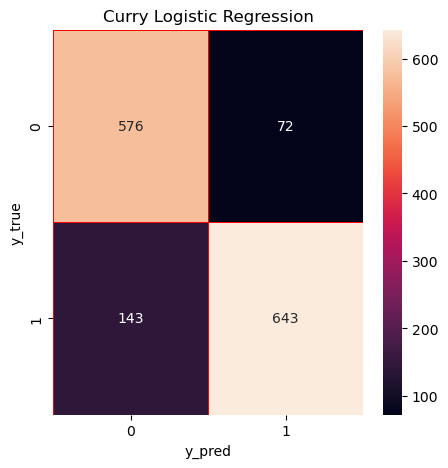
\includegraphics[width=\linewidth, height=0.45\textheight]{E_Logistic1.png}
		\end{subfigure}
		\begin{subfigure}[b]{0.45\textwidth}
			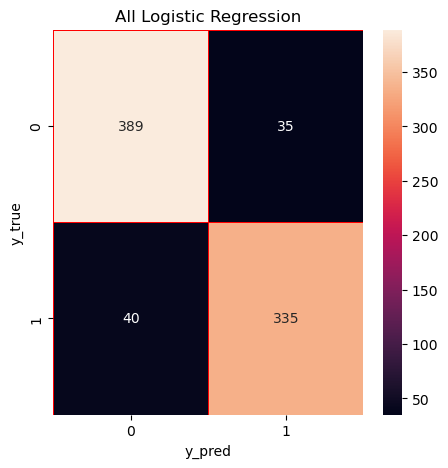
\includegraphics[width=\linewidth, height=0.45\textheight]{E_Logistic_all.png}
		\end{subfigure}
		
		\begin{subfigure}[b]{0.45\textwidth}
			\includegraphics[width=\linewidth, height=0.45\textheight]{E_Logistic1_scatter.png}
		\end{subfigure}
		\begin{subfigure}[b]{0.45\textwidth}
			\includegraphics[width=\linewidth, height=0.45\textheight]{E_Logistic_all_scatter.png}
		\end{subfigure}
	\end{figure}
\end{frame}

\begin{frame}
	\frametitle{K--najbliższych sąsiadów}
	\begin{figure}
		\begin{subfigure}[b]{0.45\textwidth}
			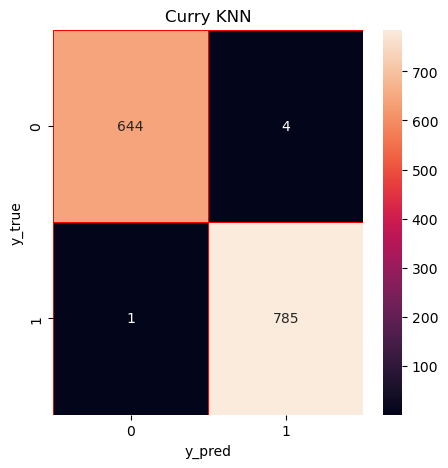
\includegraphics[width=\linewidth, height=0.45\textheight]{E_KNN1.png}
		\end{subfigure}
		\begin{subfigure}[b]{0.45\textwidth}
			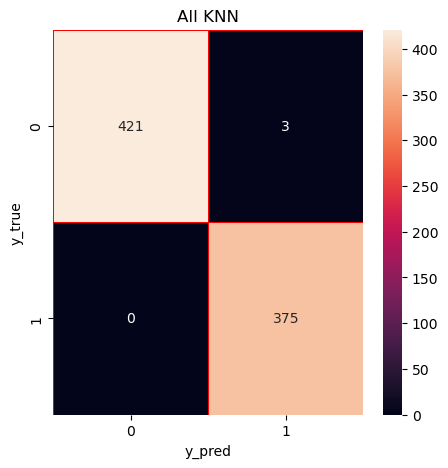
\includegraphics[width=\linewidth, height=0.45\textheight]{E_KNN_all.png}
		\end{subfigure}
		
		\begin{subfigure}[b]{0.45\textwidth}
			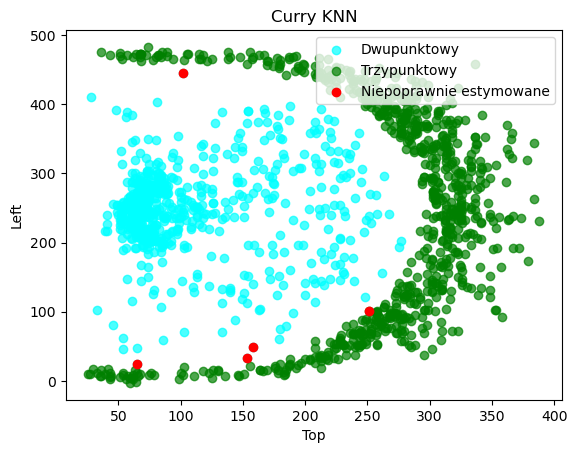
\includegraphics[width=\linewidth, height=0.45\textheight]{E_KNN1_scatter.png}
		\end{subfigure}
		\begin{subfigure}[b]{0.45\textwidth}
			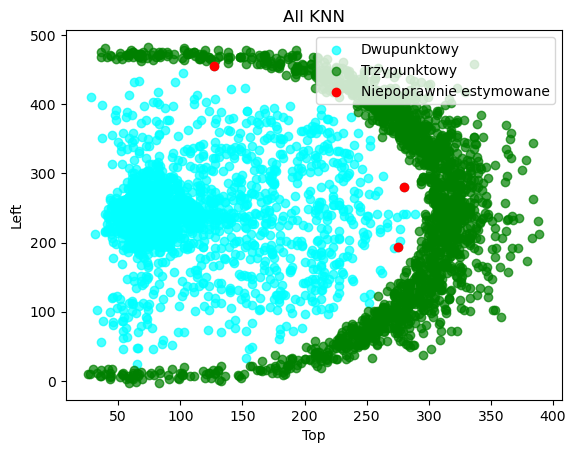
\includegraphics[width=\linewidth, height=0.45\textheight]{E_KNN_all_scatter.png}
		\end{subfigure}
	\end{figure}
\end{frame}

\begin{frame}
	\frametitle{Drzewa}
	\begin{figure}
		\begin{subfigure}[b]{0.45\textwidth}
			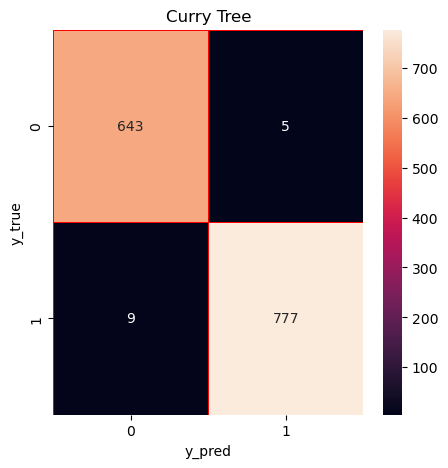
\includegraphics[width=\linewidth, height=0.45\textheight]{E_Tree1.png}
		\end{subfigure}
		\begin{subfigure}[b]{0.45\textwidth}
			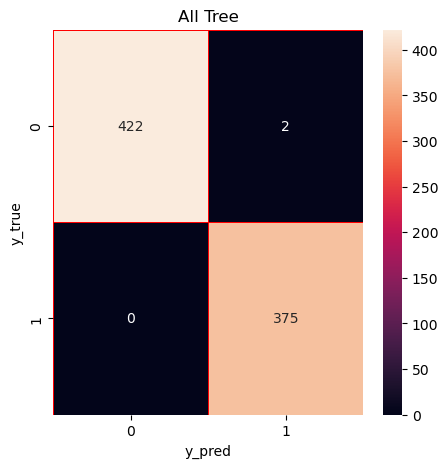
\includegraphics[width=\linewidth, height=0.45\textheight]{E_Tree_all.png}
		\end{subfigure}
		
		\begin{subfigure}[b]{0.45\textwidth}
			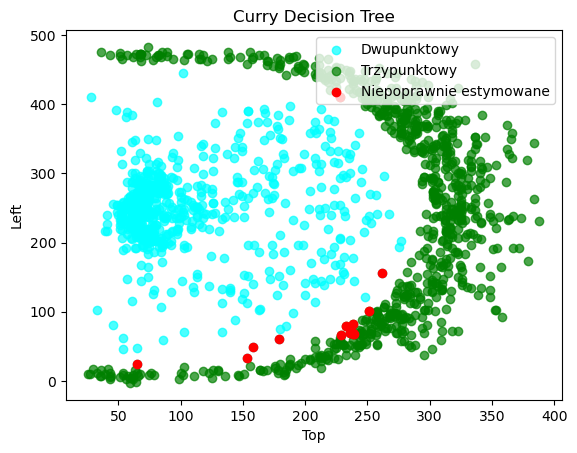
\includegraphics[width=\linewidth, height=0.45\textheight]{E_Tree1_scatter.png}
		\end{subfigure}
		\begin{subfigure}[b]{0.45\textwidth}
			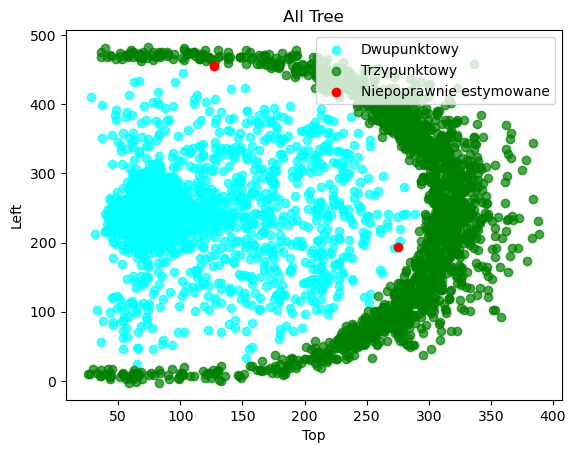
\includegraphics[width=\linewidth, height=0.45\textheight]{E_Tree_all_scatter.png}
		\end{subfigure}
	\end{figure}
\end{frame}
	\section{Wdrożenie}
		\begin{frame}
			\frametitle{Wdrożenie -- Wnioski}
			\begin{itemize}
				\item Nie jest potrzebne konstruowanie bardziej złożonych modeli obliczeniowo, gdyż te proste działają bardzo dobrze
				\item KNN radzi sobie najlepiej na danych zawodników których nie zna, natomiast drzewo decyzyjne na nowych akcjach zawodników, których już zna, regresja logistyczna odstaje od dwóch powyższych
				\item Drzewo będzie miało dużą głębokość, przez co będzie złożone obliczeniowo, wynika to z owalnego kształtu danych.
				\item Link do Githuba: \textit{\url{https://github.com/MichalBrodackiPJA/Eksploracja-i-Wizualizacja-Danych/tree/master/Projekt_koncowy}}
			\end{itemize}
			
				\vspace{0.5cm}
			
			\centering\Large{Dziękuję za uwagę!}
			
		\end{frame}
		
\end{document}